\section{Survey som Dataindsamling}
For at kunne udlede en sammenhæng mellem stemningsleje og social aktivitet skal der udover målinger af den sociale aktivitet også bruges subjekt data fra patienten.
Til dette formål skal der konstrueres et modul der kan stille spørgsmål til patienten på varierende tidspunkter.
\mikael{Omformuler så 'subjektiv' ikke bruges}

\subsection{Spørgsmål}\label{survey:spg}
Da der er forskellige metoder til at konsultere en patient om sit stemningsleje er det nødvendigt at kunne stille spørgsmål på forskellige måder.
Der er udvalgt tre typer spørgsmål som vi mener dækker de behov der i forhold til at udspørge patienten både om sin sociale færden og om sit stemningsleje.
Disse typer vil i det følgende blive gennemgået med eksempler på hvilke relevante metoder fra psykologien de kan bruges til.

\paragraph{Multiple choice}
Stemningsregistrering, \cref{stemningsleje::stemningsregistrering}, bruger en skala fra ``svær depression'' til ``svær mani'' til at holde øje med hvor patientens stemningsleje.
Det skal både være muligt at lave spørgsmål hvor man kun kan vælge en mulighed og spørgsmål hvor man kan vælge flere svarmuligheder.
Jævnfør stemningregistrering skalaen skal der kunne tilknyttes en farve til de forkellige muligheder.

\stefan{Hamilton}

\paragraph{Tekst}
For at give mulighed for at patienten kan skrive dagbog \stefan{ref til Måling af stemningsleje} skal der bruges en spørgsmålstype der kan vise en kort tekst som besvares med en tekst fra et tekstfelt.
På denne måde kan der både skrives regulær dagbog, og der kan stilles konkrete spørgsmål såsom ``Hvordan har du ageret socialt i dag?''.

\paragraph{Skala}
I metoden PANAS \stefan{ref til Måling af stemningsleje}stilles patienten et spørgsmål om i hvor høj grad han har følt en bestemt følelse i en vis tidsperiode.
Dette besvares så på en skala fra et til fem.

Vi har altså behov for et spørgsmål der kan besvares med en numerisk skala med mulighed for at sætte labels på skalaen.

\subsection{Implementation af de forskellige typer svar\bruno{Eller spørgsmål - hvad vi nu finder ud af}}
Gennem dette afsnit vil der blive refereret til \cref{stemreg::spoergsmaal}, som er en eksempel implementation af metoden: stemningsregistrering beskrevet i \cref{stemningsleje::stemningsregistrering}.
De tre typer af spørgsmål, beskrevet i \cref{krav::typer}, er blevet implementeret, eksempler på brug kan ses på \cref{stemreg::spoergsmaal}.
På \cref{stemreg::stemningsleje} kan ses en multiple choice spørgsmål hvor der kan vælges flere svarmuligheder.
Dette spørgsmål findes også i en variant hvor man kun kan vælge en mulighed, indikeret ved runde svarbokse (radio buttons).

\Cref{stemreg::soevn} viser et spørgsmål der besvares ved en skala. 
Spørgsmålene har to labels et for minimum og et for maksimum.

\Cref{stemreg::notater_vaegt} viser et spørgsmål der skal besvares ved en tekst. 


\begin{figure}
	\centering
	\begin{subfigure}[b]{0.45\textwidth}
		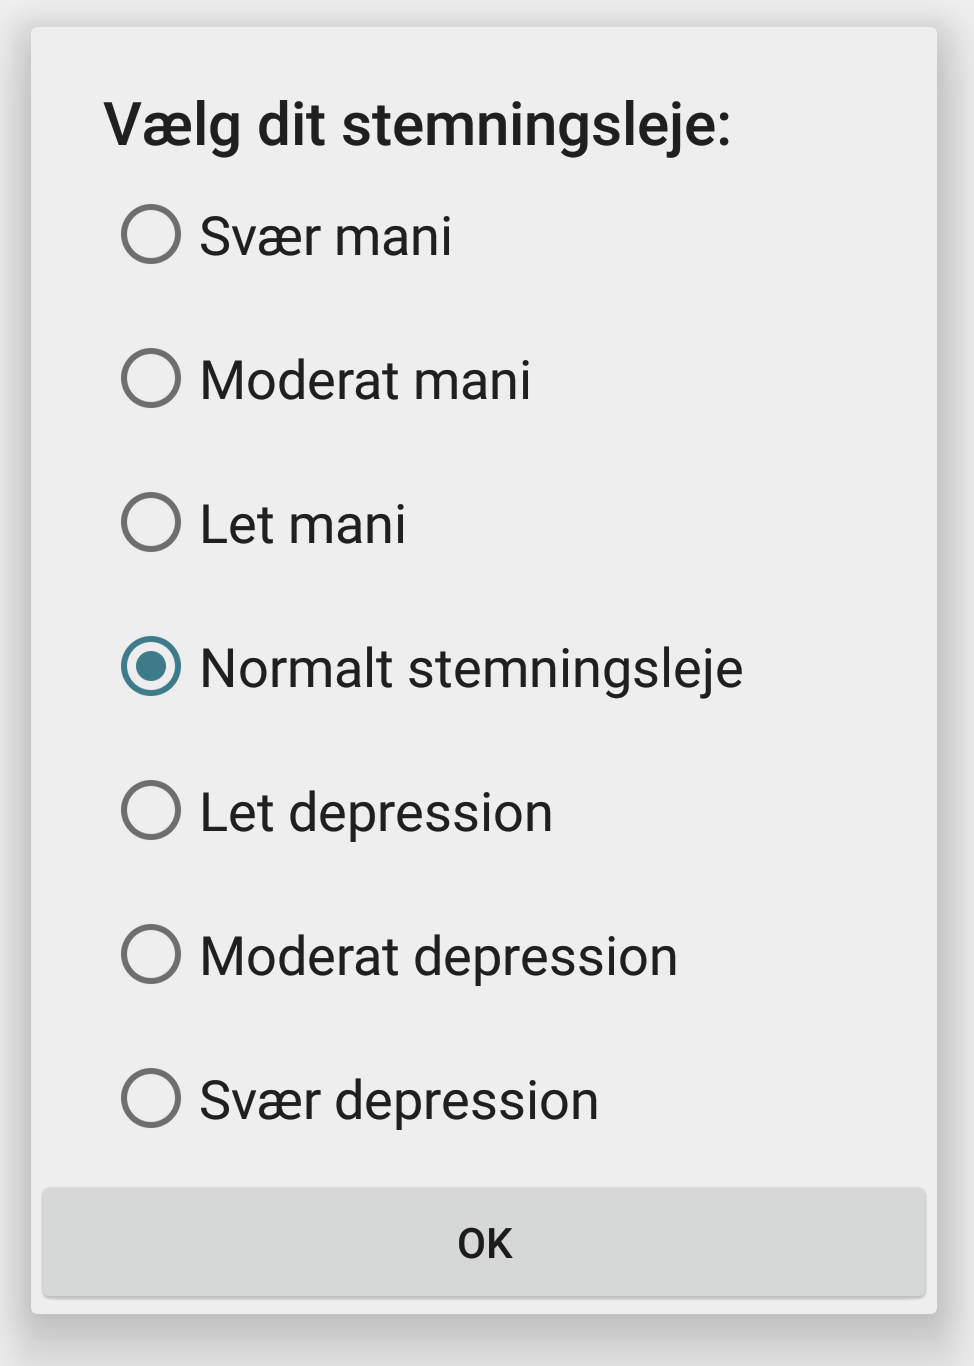
\includegraphics[width=\textwidth]{stemningsregistrering_eksempel/stemningsleje}
		\caption{Multiple choice}\label{stemreg::stemningsleje}
	\end{subfigure}
	\hfill
\begin{minipage}[b]{0.45\textwidth}
	\begin{subfigure}[b]{\textwidth}
		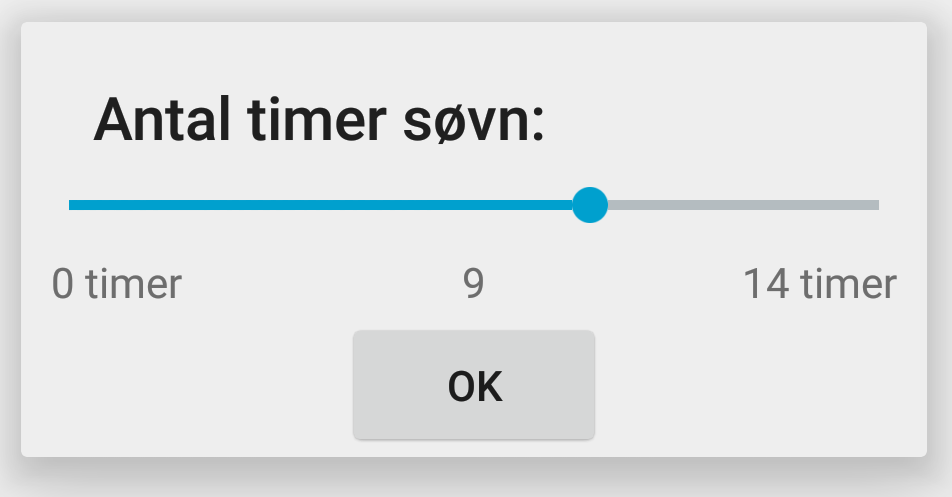
\includegraphics[width=\textwidth]{stemningsregistrering_eksempel/soevn}
		\caption{Skala}\label{stemreg::soevn}
	\end{subfigure}
	\newline 
	\begin{subfigure}[b]{\textwidth}
		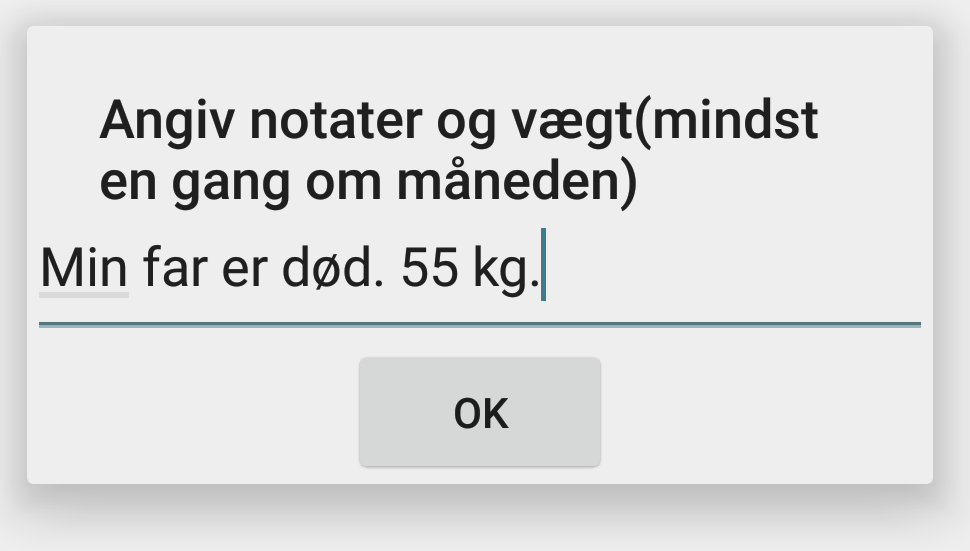
\includegraphics[width=\textwidth]{stemningsregistrering_eksempel/notater_vaegt}
		\caption{Tekst}\label{stemreg::notater_vaegt}
	\end{subfigure}	
\end{minipage}	
	\caption{Tre af de fem spørgsmål der bruges i metoden: stemningsregistrering( \cref{stemningsleje::stemningsregistrering}), for at vise de tre spørgsmåls typer.}\label{stemreg::spoergsmaal}
\end{figure}

\subsection{Scheduler}
For at kunne stille spørgsmål så fleksibelt som muligt er der blevet konstrueret en scheduler.
Stemningsregistrering og dagbog skal ske én gang om dagen, mens PANAS spørgsmål sagtens kan spredes ud over dagen for at få et bredere billede af patientens tilstand.


\paragraph{Notifikationer}
For ikke at forstyrre brugerens hverdag for meget bruger vi en notifikation til at advisere om et forestående spørgsmål.
Notifikationen indeholder spørgsmålsteksten, så patienten kan vurdere om han har tid til at besvare spørgsmålet.
Eksempler på disse notifikationer kan ses på \cref{noti}.

\begin{figure}
	\centering
	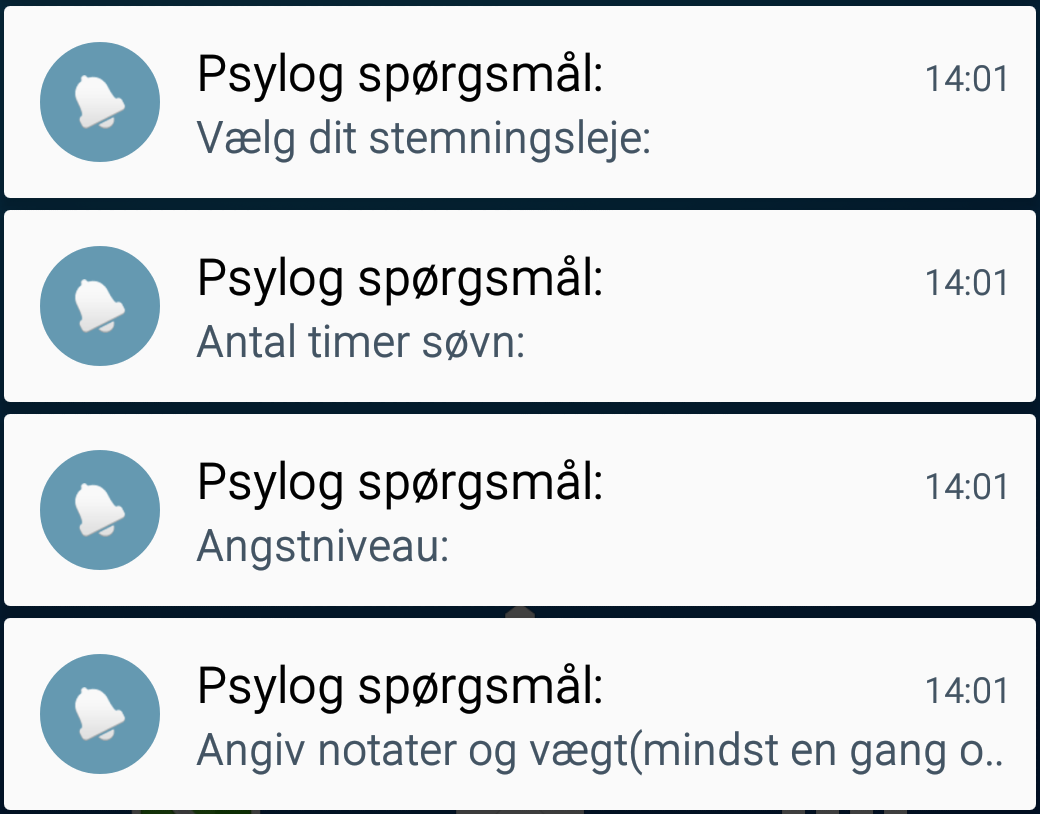
\includegraphics[width=0.6\textwidth]{stemningsregistrering_eksempel/notification_bar}
	\caption{Fire notifikationer sendt af Survey}\label{noti}
\end{figure}

Når der trykkes på notifikationen dukker spørgsmålet op i en dialogboks hvor patientes svar kan indføres.

For at gøre systemet endnu mere fleksibelt skal der være mulighed for at kunne udskyde et spørgsmål.
På denne måde har patienten fuld kontrol over hvornår han svarer, uden at være nødt til at skulle afbryde det han er i gang med.
Dette er endnu ikke implementeret.